% ============================================================
%  SCHOLA DOMESTICA — Level 1, Week 1, Lesson 3
%  Topic: Numbers 4 and 5
% ============================================================
\documentclass[12pt,letterpaper]{article}
\usepackage[top=1in,bottom=1in,left=1in,right=1in]{geometry}
\usepackage{fontspec}\usepackage{graphicx}\usepackage{xcolor}
\usepackage{mdframed}\usepackage{tikz}\usepackage{fancyhdr}\usepackage{parskip}
\usetikzlibrary{shapes.geometric}
\setmainfont{EB Garamond}[Ligatures=TeX,Numbers=OldStyle]
\definecolor{sd-blue}{RGB}{60,100,160}\definecolor{sd-gold}{RGB}{180,140,50}
\definecolor{sd-light}{RGB}{245,242,235}\definecolor{sd-green}{RGB}{70,130,80}
\pagestyle{fancy}\fancyhf{}
\fancyhead[L]{\small\color{sd-blue}\textit{Schola Domestica Mathematics}}
\fancyhead[R]{\small\color{sd-blue}\textit{Level~1 \(\cdot\) Week~1 \(\cdot\) Lesson~3}}
\fancyfoot[C]{\small\color{sd-blue}1}
\renewcommand{\headrulewidth}{0.4pt}
\newmdenv[backgroundcolor=sd-light,linecolor=sd-blue,linewidth=1pt,
  innerleftmargin=10pt,innerrightmargin=10pt,innertopmargin=8pt,
  innerbottommargin=8pt,roundcorner=4pt]{instructbox}
\newmdenv[backgroundcolor=white,linecolor=sd-green,linewidth=1.5pt,
  innerleftmargin=10pt,innerrightmargin=10pt,innertopmargin=8pt,
  innerbottommargin=8pt,roundcorner=4pt]{checkbox}
\newcommand{\ansblank}{\underline{\hspace{1.6cm}}}
\newcounter{probnum}
\newcommand{\prob}{\stepcounter{probnum}\noindent\textbf{\arabic{probnum}.}\quad}
\newcommand{\onestar}{
\begin{tikzpicture}[baseline=-0.1cm]
  \node[star,star points=5,star point ratio=2.5,fill=sd-gold,
        draw=sd-gold!80!black,minimum size=0.9cm]{};
  \end{tikzpicture}}
\newcommand{\onedot}{
\begin{tikzpicture}[baseline=-0.05cm]
  \fill[sd-blue](0,0)circle(0.22cm);
  \end{tikzpicture}}
\begin{document}
\begin{center}
  {\color{sd-blue}\Large\bfseries Schola Domestica Mathematics — Level~1}\\[4pt]
  {\color{sd-blue}\rule{\linewidth}{1.5pt}}\\[6pt]
  {\LARGE\bfseries Lesson 3 \quad|\quad Numbers 4 and 5}\\[4pt]
  {\color{sd-gold}\rule{\linewidth}{0.8pt}}
\end{center}
\vspace{4pt}
\begin{instructbox}
\noindent\textbf{\color{sd-blue}Instruction:}\\[4pt]
Today we meet \textbf{4} and \textbf{5}.
Hold up four fingers, then add one more — that is five.
Five fingers fill one whole hand!
\end{instructbox}
\vspace{8pt}
\noindent\textbf{\color{sd-blue}Trace and write:}
\vspace{4pt}
\begin{center}
\begin{tabular}{|c|c|c|c|c|c|c|c|}
\hline
\rule{0pt}{26pt}{\Huge\color{sd-blue!40}4}&{\Huge\phantom{4}}&{\Huge\phantom{4}}&{\Huge\phantom{4}}&
{\Huge\color{sd-blue!40}5}&{\Huge\phantom{5}}&{\Huge\phantom{5}}&{\Huge\phantom{5}}\\
\hline
\end{tabular}
\end{center}
\vspace{4pt}{\color{sd-gold}\rule{\linewidth}{0.5pt}}\vspace{4pt}
\noindent\textbf{\color{sd-blue}Practice}\vspace{4pt}

\prob Count the dots.\quad\onedot\onedot\onedot\onedot\quad\ansblank

\vspace{8pt}
\prob Count the dots.\quad\onedot\onedot\onedot\onedot\onedot\quad\ansblank

\vspace{8pt}
\prob How many? \quad
\IfFileExists{stars_5.jpg}{
\includegraphics[height=1.4cm]{stars_5.jpg}}{%
  \onestar\onestar\onestar\onestar\onestar}
\quad\ansblank

\vspace{8pt}
\prob How many? \quad
\IfFileExists{apples_4.jpg}{
\includegraphics[height=1.4cm]{apples_4.jpg}}{%
  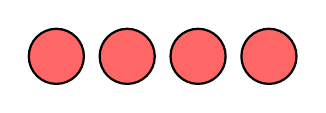
\begin{tikzpicture}[baseline=0]
    \foreach \x in {0,1,2,3}\draw[fill=red!60,thick](\x*0.9,0)circle(0.35);
  \end{tikzpicture}}
\quad\ansblank

\vspace{8pt}
\prob Circle the correct number for this group: \quad
  \IfFileExists{ducks_4.jpg}{
\includegraphics[height=1.4cm]{ducks_4.jpg}}{%
    
\begin{tikzpicture}[baseline=0]
      \foreach \x in {0,1,2,3}\draw[fill=yellow!70,thick](\x*0.9,0)ellipse(0.35 and 0.25);
    \end{tikzpicture}}
  \quad{\Large 3 \quad \textbf{4} \quad 5}

\vspace{8pt}
\prob Draw \textbf{4} flowers in the box:
\vspace{2pt}
\noindent\fbox{\rule{0pt}{2cm}\hspace{9cm}}

\vspace{8pt}
\prob \textit{(Teacher reads)} A bird had 3 eggs in her nest.
She laid 2 more eggs. Now how many eggs are there? \quad\ansblank
\textit{(Hint: count all the eggs.)}

\vspace{8pt}
\prob Write the numbers 1 through 5 in order:\\[4pt]
\hspace{1cm}\ansblank\quad\ansblank\quad\ansblank\quad\ansblank\quad\ansblank

\vspace{8pt}
\prob What number comes right after 4? \quad\ansblank

\vspace{6pt}
\prob What number comes right before 5? \quad\ansblank

\vspace{6pt}{\color{sd-gold}\rule{\linewidth}{0.5pt}}\vspace{4pt}
\begin{checkbox}
\noindent\textbf{\color{sd-green}Knowledge Check}\\[4pt]
\setcounter{probnum}{0}
\prob \IfFileExists{stars_4.jpg}{
\includegraphics[height=1.2cm]{stars_4.jpg}}{%
  \onestar\onestar\onestar\onestar}\quad\ansblank\\[8pt]
\prob How many fingers on one hand? \quad\ansblank
\end{checkbox}
\vfill
\noindent{\color{sd-blue}$\bigstar$ \textbf{Enrichment:}}
In Latin: \textit{ūnus, duo, tr\={e}s, quattuor, quīnque}.
Can you say all five?
\vspace{4pt}\hrule\vspace{2pt}
{\footnotesize\color{gray}\textit{Teacher note: Five is a critical anchor number. Spend extra time if needed.}}
\end{document}\hline
\end{tabular}
\end{center}
\vspace{4pt}{\color{sd-gold}\rule{\linewidth}{0.5pt}}\vspace{4pt}
\noindent\textbf{\color{sd-blue}Practice}\vspace{4pt}

\prob Count the dots.\quad\onedot\onedot\onedot\onedot\quad\ansblank

\vspace{8pt}
\prob Count the dots.\quad\onedot\onedot\onedot\onedot\onedot\quad\ansblank

\vspace{8pt}
\prob How many? \quad
\IfFileExists{stars_5.jpg}{
\includegraphics[height=1.4cm]{stars_5.jpg}}{%
  \onestar\onestar\onestar\onestar\onestar}
\quad\ansblank

\vspace{8pt}
\prob How many? \quad
\IfFileExists{apples_4.jpg}{
\includegraphics[height=1.4cm]{apples_4.jpg}}{%
  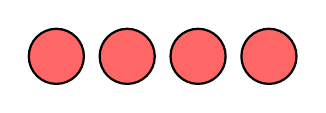
\begin{tikzpicture}[baseline=0]
    \foreach \x in {0,1,2,3}\draw[fill=red!60,thick](\x*0.9,0)circle(0.35);
  \end{tikzpicture}}
\quad\ansblank

\vspace{8pt}
\prob Circle the correct number for this group: \quad
  \IfFileExists{ducks_4.jpg}{
\includegraphics[height=1.4cm]{ducks_4.jpg}}{%
    
\begin{tikzpicture}[baseline=0]
      \foreach \x in {0,1,2,3}\draw[fill=yellow!70,thick](\x*0.9,0)ellipse(0.35 and 0.25);
    \end{tikzpicture}}
  \quad{\Large 3 \quad \textbf{4} \quad 5}

\vspace{8pt}
\prob Draw \textbf{4} flowers in the box:
\vspace{2pt}
\noindent\fbox{\rule{0pt}{2cm}\hspace{9cm}}

\vspace{8pt}
\prob \textit{(Teacher reads)} A bird had 3 eggs in her nest.
She laid 2 more eggs. Now how many eggs are there? \quad\ansblank
\textit{(Hint: count all the eggs.)}

\vspace{8pt}
\prob Write the numbers 1 through 5 in order:\\[4pt]
\hspace{1cm}\ansblank\quad\ansblank\quad\ansblank\quad\ansblank\quad\ansblank

\vspace{8pt}
\prob What number comes right after 4? \quad\ansblank

\vspace{6pt}
\prob What number comes right before 5? \quad\ansblank

\vspace{6pt}{\color{sd-gold}\rule{\linewidth}{0.5pt}}\vspace{4pt}
\begin{checkbox}
\noindent\textbf{\color{sd-green}Knowledge Check}\\[4pt]
\setcounter{probnum}{0}
\prob \IfFileExists{stars_4.jpg}{
\includegraphics[height=1.2cm]{stars_4.jpg}}{%
  \onestar\onestar\onestar\onestar}\quad\ansblank\\[8pt]
\prob How many fingers on one hand? \quad\ansblank
\end{checkbox}
\vfill
\noindent{\color{sd-blue}$\bigstar$ \textbf{Enrichment:}}
In Latin: \textit{ūnus, duo, tr\={e}s, quattuor, quīnque}.
Can you say all five?
\vspace{4pt}\hrule\vspace{2pt}
{\footnotesize\color{gray}\textit{Teacher note: Five is a critical anchor number. Spend extra time if needed.}}
\end{document}


% ============================================================
%  SCHOLA DOMESTICA — Level 1, Week 1, Lesson 4
%  Topic: Comparing Groups — More, Fewer, Same (Numbers 1–5)
% ============================================================
% Save as: sd_L1_W1_L4.tex

\documentclass[12pt,letterpaper]{article}
\usepackage[top=1in,bottom=1in,left=1in,right=1in]{geometry}
\usepackage{fontspec}\usepackage{graphicx}\usepackage{xcolor}
\usepackage{mdframed}\usepackage{tikz}\usepackage{fancyhdr}\usepackage{parskip}
\usetikzlibrary{shapes.geometric}
\setmainfont{EB Garamond}[Ligatures=TeX,Numbers=OldStyle]
\definecolor{sd-blue}{RGB}{60,100,160}\definecolor{sd-gold}{RGB}{180,140,50}
\definecolor{sd-light}{RGB}{245,242,235}\definecolor{sd-green}{RGB}{70,130,80}
\pagestyle{fancy}\fancyhf{}
\fancyhead[L]{\small\color{sd-blue}\textit{Schola Domestica Mathematics}}
\fancyhead[R]{\small\color{sd-blue}\textit{Level~1 \(\cdot\) Week~1 \(\cdot\) Lesson~4}}
\fancyfoot[C]{\small\color{sd-blue}1}
\renewcommand{\headrulewidth}{0.4pt}
\newmdenv[backgroundcolor=sd-light,linecolor=sd-blue,linewidth=1pt,
  innerleftmargin=10pt,innerrightmargin=10pt,innertopmargin=8pt,
  innerbottommargin=8pt,roundcorner=4pt]{instructbox}
\newmdenv[backgroundcolor=white,linecolor=sd-green,linewidth=1.5pt,
  innerleftmargin=10pt,innerrightmargin=10pt,innertopmargin=8pt,
  innerbottommargin=8pt,roundcorner=4pt]{checkbox}
\newcommand{\ansblank}{\underline{\hspace{1.8cm}}}
\newcounter{probnum}
\newcommand{\prob}{\stepcounter{probnum}\noindent\textbf{\arabic{probnum}.}\quad}
\newcommand{\onestar}{
\begin{tikzpicture}[baseline=-0.1cm]
  \node[star,star points=5,star point ratio=2.5,fill=sd-gold,
        draw=sd-gold!80!black,minimum size=0.9cm]{};
  \end{tikzpicture}}
\begin{document}
\begin{center}
  {\color{sd-blue}\Large\bfseries Schola Domestica Mathematics — Level~1}\\[4pt]
  {\color{sd-blue}\rule{\linewidth}{1.5pt}}\\[6pt]
  {\LARGE\bfseries Lesson 4 \quad|\quad More, Fewer, or the Same?}\\[4pt]
  {\color{sd-gold}\rule{\linewidth}{0.8pt}}
\end{center}
\vspace{4pt}
\begin{instructbox}
\noindent\textbf{\color{sd-blue}Instruction:}\\[4pt]
When one group has more objects than another, we say it has \textbf{more}.
When it has fewer, we say \textbf{fewer}.
When they match exactly, we say \textbf{same}.
\end{instructbox}
\vspace{8pt}
\noindent\textbf{\color{sd-blue}Practice}
\vspace{6pt}

\prob Which group has \textbf{more}? Circle it.\\[4pt]
\begin{tabular}{lcl}
Group A: & \onestar\onestar\onestar & (3 stars)\\[4pt]
Group B: & \onestar\onestar\onestar\onestar\onestar & (5 stars)
\end{tabular}

\vspace{10pt}
\prob Which group has \textbf{fewer}? Circle it.\\[4pt]
\begin{tabular}{lcl}
Group A: &
\IfFileExists{apples_4.jpg}{
\includegraphics[height=1.3cm]{apples_4.jpg}}{%
  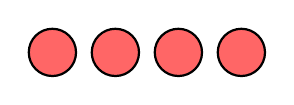
\begin{tikzpicture}[baseline=0]\foreach\x in{0,1,2,3}\draw[fill=red!60,thick](\x*0.8,0)circle(0.3);\end{tikzpicture}}
& (4 apples)\\[4pt]
Group B: &
\IfFileExists{apples_2.jpg}{
\includegraphics[height=1.3cm]{apples_2.jpg}}{%
  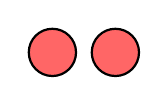
\begin{tikzpicture}[baseline=0]\foreach\x in{0,1}\draw[fill=red!60,thick](\x*0.8,0)circle(0.3);\end{tikzpicture}}
& (2 apples)
\end{tabular}

\vspace{10pt}
\prob Are these groups the \textbf{same}? Write yes or no.\\[4pt]
\begin{tabular}{lcl}
Group A: & \onestar\onestar\onestar & \\[4pt]
Group B: & \onestar\onestar\onestar &
\end{tabular}\quad\ansblank

\vspace{10pt}
\prob Draw a group with the \textbf{same} number as these ducks:\\[4pt]
\IfFileExists{ducks_4.jpg}{
\includegraphics[height=1.6cm]{ducks_4.jpg}}{%
  
\begin{tikzpicture}[baseline=0]\foreach\x in{0,1,2,3}\draw[fill=yellow!70,thick](\x*0.9,0)ellipse(0.35 and 0.25);\end{tikzpicture}}\\[6pt]
\noindent\fbox{\rule{0pt}{2.2cm}\hspace{9cm}}

\vspace{10pt}
\prob \textit{(Teacher reads)} A pond has 3 goldfish. A bowl has 5 goldfish.
Which has more? \quad\ansblank

\vspace{10pt}
\prob Write the number that is \textbf{more}: \quad 2 \quad or \quad 4 \quad $\longrightarrow$ \quad\ansblank

\vspace{10pt}
\prob Write the number that is \textbf{fewer}: \quad 5 \quad or \quad 3 \quad $\longrightarrow$ \quad\ansblank

\vspace{10pt}
\prob \textit{(Teacher reads)} Sara has 2 flowers. Tom has 2 flowers.
Do they have the same? \quad\ansblank

\vspace{8pt}{\color{sd-gold}\rule{\linewidth}{0.5pt}}\vspace{4pt}
\begin{checkbox}
\noindent\textbf{\color{sd-green}Knowledge Check}\\[4pt]
\setcounter{probnum}{0}
\prob Which is more: 3 or 5? \quad\ansblank\\[8pt]
\prob Which is fewer: 4 or 1? \quad\ansblank
\end{checkbox}
\vfill
\noindent{\color{sd-blue}$\bigstar$ \textbf{Enrichment:}}
In Latin: \textit{plus} means more and \textit{minus} means less (fewer).
You already know two math words in Latin!
\vspace{4pt}\hrule\vspace{2pt}
{\footnotesize\color{gray}\textit{Teacher note: Use physical objects to compare groups before the worksheet if the concept is new.}}
\end{document}


% ============================================================
%  SCHOLA DOMESTICA — Level 1, Week 1, Lesson 5
%  Topic: Numbers 1–5 Review & Ordering
%  (Friday lesson — slightly lighter, joyful consolidation)
% ============================================================
% Save as: sd_L1_W1_L5.tex

\documentclass[12pt,letterpaper]{article}
\usepackage[top=1in,bottom=1in,left=1in,right=1in]{geometry}
\usepackage{fontspec}\usepackage{graphicx}\usepackage{xcolor}
\usepackage{mdframed}\usepackage{tikz}\usepackage{fancyhdr}\usepackage{parskip}
\usetikzlibrary{shapes.geometric}
\setmainfont{EB Garamond}[Ligatures=TeX,Numbers=OldStyle]
\definecolor{sd-blue}{RGB}{60,100,160}\definecolor{sd-gold}{RGB}{180,140,50}
\definecolor{sd-light}{RGB}{245,242,235}\definecolor{sd-green}{RGB}{70,130,80}
\pagestyle{fancy}\fancyhf{}
\fancyhead[L]{\small\color{sd-blue}\textit{Schola Domestica Mathematics}}
\fancyhead[R]{\small\color{sd-blue}\textit{Level~1 \(\cdot\) Week~1 \(\cdot\) Lesson~5}}
\fancyfoot[C]{\small\color{sd-blue}1}
\renewcommand{\headrulewidth}{0.4pt}
\newmdenv[backgroundcolor=sd-light,linecolor=sd-blue,linewidth=1pt,
  innerleftmargin=10pt,innerrightmargin=10pt,innertopmargin=8pt,
  innerbottommargin=8pt,roundcorner=4pt]{instructbox}
\newmdenv[backgroundcolor=white,linecolor=sd-green,linewidth=1.5pt,
  innerleftmargin=10pt,innerrightmargin=10pt,innertopmargin=8pt,
  innerbottommargin=8pt,roundcorner=4pt]{checkbox}
\newcommand{\ansblank}{\underline{\hspace{1.8cm}}}
\newcounter{probnum}
\newcommand{\prob}{\stepcounter{probnum}\noindent\textbf{\arabic{probnum}.}\quad}
\newcommand{\onestar}{
\begin{tikzpicture}[baseline=-0.1cm]
  \node[star,star points=5,star point ratio=2.5,fill=sd-gold,
        draw=sd-gold!80!black,minimum size=0.9cm]{};
  \end{tikzpicture}}
\begin{document}
\begin{center}
  {\color{sd-blue}\Large\bfseries Schola Domestica Mathematics — Level~1}\\[4pt]
  {\color{sd-blue}\rule{\linewidth}{1.5pt}}\\[6pt]
  {\LARGE\bfseries Lesson 5 \quad|\quad Numbers 1–5: Review \& Ordering}\\[4pt]
  {\color{sd-gold}\rule{\linewidth}{0.8pt}}
\end{center}
\vspace{4pt}
\begin{instructbox}
\noindent\textbf{\color{sd-blue}Instruction:}\\[4pt]
Well done this week!
Today we practice everything we have learned about numbers 1 through 5.
Let us count, write, compare, and order — you know how!
\end{instructbox}
\vspace{8pt}
\noindent\textbf{\color{sd-blue}Practice}
\vspace{6pt}

\prob Count and write the number.

\vspace{4pt}
\begin{tabular}{ccccc}
\IfFileExists{stars_1.jpg}{
\includegraphics[height=1.3cm]{stars_1.jpg}}{\onestar} &
\IfFileExists{stars_3.jpg}{
\includegraphics[height=1.3cm]{stars_3.jpg}}{\onestar\onestar\onestar} &
\IfFileExists{stars_5.jpg}{
\includegraphics[height=1.3cm]{stars_5.jpg}}{\onestar\onestar\onestar\onestar\onestar} &
\IfFileExists{stars_2.jpg}{
\includegraphics[height=1.3cm]{stars_2.jpg}}{\onestar\onestar} &
\IfFileExists{stars_4.jpg}{
\includegraphics[height=1.3cm]{stars_4.jpg}}{\onestar\onestar\onestar\onestar} \\[4pt]
\ansblank & \ansblank & \ansblank & \ansblank & \ansblank
\end{tabular}

\vspace{10pt}
\prob Put these numbers in order from smallest to largest:\\[4pt]
\hspace{2cm}{\Large 4 \quad 1 \quad 3 \quad 5 \quad 2}\\[4pt]
\hspace{2cm}\ansblank\quad\ansblank\quad\ansblank\quad\ansblank\quad\ansblank

\vspace{10pt}
\prob Write the missing numbers:
\vspace{4pt}
\begin{center}
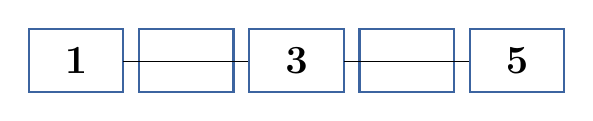
\begin{tikzpicture}
  \foreach \n/\v in {1/1,2/?,3/3,4/?,5/5}{
    \draw[sd-blue,thick] (\n*1.4-1.4,0) rectangle (\n*1.4-0.2,0.8);
    \node at (\n*1.4-0.8,0.4) {\Large\ifnum\n=2 \ansblank\else\ifnum\n=4 \ansblank\else\textbf{\v}\fi\fi};
  }
\end{tikzpicture}
\end{center}

\vspace{10pt}
\prob Draw a line to match each number to the correct group.

\vspace{6pt}
\begin{tabular}{p{3cm} p{3cm} p{5cm}}
\textbf{2} & \hspace{1cm}$\longleftrightarrow$ &
  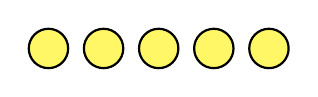
\begin{tikzpicture}[baseline=0]\foreach\x in{0,1,2,3,4}\draw[fill=yellow!60,thick](\x*0.7,0)circle(0.25);\end{tikzpicture}\\[10pt]
\textbf{5} & \hspace{1cm}$\longleftrightarrow$ &
  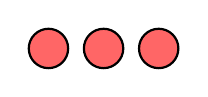
\begin{tikzpicture}[baseline=0]\foreach\x in{0,1,2}\draw[fill=red!60,thick](\x*0.7,0)circle(0.25);\end{tikzpicture}\\[10pt]
\textbf{3} & \hspace{1cm}$\longleftrightarrow$ &
  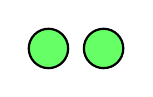
\begin{tikzpicture}[baseline=0]\foreach\x in{0,1}\draw[fill=green!60,thick](\x*0.7,0)circle(0.25);\end{tikzpicture}
\end{tabular}

\vspace{10pt}
\prob Which number is the greatest? \quad 1 \quad 3 \quad 5 \quad 2 \quad 4 \quad $\longrightarrow$ \quad\ansblank

\vspace{10pt}
\prob \textit{(Teacher reads)} Five rabbits were in the garden.
Two hopped away. How many stayed? \quad\ansblank
\textit{(Use fingers to figure it out!)}

\vspace{10pt}
\prob \IfFileExists{happy_stars.jpg}{\includegraphics[height=1.8cm]{happy_stars.jpg}}{%
  
\begin{tikzpicture}
    \foreach \x in {0,...,4}
      \node[star,star points=5,star point ratio=2.5,fill=sd-gold,draw=sd-gold!70!black,
            minimum size=1.1cm] at (\x*1.3,0) {};
  \end{tikzpicture}}\\[4pt]
How many happy stars? \quad\ansblank \quad
Write the number in the box: \fbox{\rule{0pt}{1cm}\hspace{1.2cm}}

\vspace{10pt}
\prob Write the numbers 1, 2, 3, 4, 5 — your neatest handwriting!\\[8pt]
\noindent\fbox{\rule{0pt}{1.8cm}\hspace{12cm}}

\vspace{8pt}{\color{sd-gold}\rule{\linewidth}{0.5pt}}\vspace{4pt}
\begin{checkbox}
\noindent\textbf{\color{sd-green}Knowledge Check}\\[4pt]
\setcounter{probnum}{0}
\prob Say the numbers 1 to 5 aloud to your teacher. \quad
  $\square$~Done\\[8pt]
\prob \onestar\onestar\onestar\quad How many? \quad\ansblank \quad
  Is that more or fewer than 5? \quad\ansblank
\end{checkbox}
\vfill
\noindent{\color{sd-blue}$\bigstar$ \textbf{Enrichment — Roman Numerals!}}\\
The Romans wrote numbers like this:\\[4pt]
\begin{tabular}{ccccc}
\textbf{I} & \textbf{II} & \textbf{III} & \textbf{IV} & \textbf{V} \\
1 & 2 & 3 & 4 & 5
\end{tabular}\\[4pt]
Try writing them yourself in the box:
\noindent\fbox{\rule{0pt}{1.2cm}\hspace{10cm}}
\vspace{4pt}\hrule\vspace{2pt}
{\footnotesize\color{gray}\textit{Teacher note: Week 1 mastery target — student identifies and writes 1–5
  without hesitation and can say which of two numbers is greater.
  If not yet solid, repeat Lesson 1 or 2 before proceeding to Week 2.}}
\end{document}
